\chapter{实验数据采集与分析}\label{experiment}

\section{仿真平台}
\subsection{ROS简介}
ROS(Robot Operating System,机器人操作系统)是为机器人软件开发的一种计算机操作系统架构,源自于斯坦福AI机器人项目。ROS能够为跨平台、跨语言的异构计算机集群提供结构化通信。ROS包括标准的操作系统环境,包括底层设备控制与管理、进程间消息传递机制和软件包管理等功能。ROS操作系统能够使开发者非常方便的构建多语言的机器人软件功能。如\ref{system} 所述,我们在ROS系统的基础上构建驱动、感知、规划、控制和决策功能模组。

\subsection{RVIZ与Gazebo}
RVIZ是ROS自带的图形化工具。在本文中,我们将轮式机器人的雷达、里程计等传感器数据以及定位、路径规划等感知和规划功能模组中间结果在RVIZ界面中进行可视化,如图\ref{rviz}所示。Gazebo是基于ROS的一款功能强大的3D 机器人仿真模拟器。我们使用Gazebo进行仿真建模,准确有效地模拟复现轮式机器人在挑战赛场地内的状态和行为,如图\ref{gazebo}所示。Gazebo通过高性能的物理引擎,对轮式机器人进行物理建模,动力学仿真,模拟真实环境下的传感器和噪声,使我们的强化学习算法获得逼近于真实环境的训练。
\begin{figure}[ht]
  \centering
  % Requires \usepackage{graphicx}
  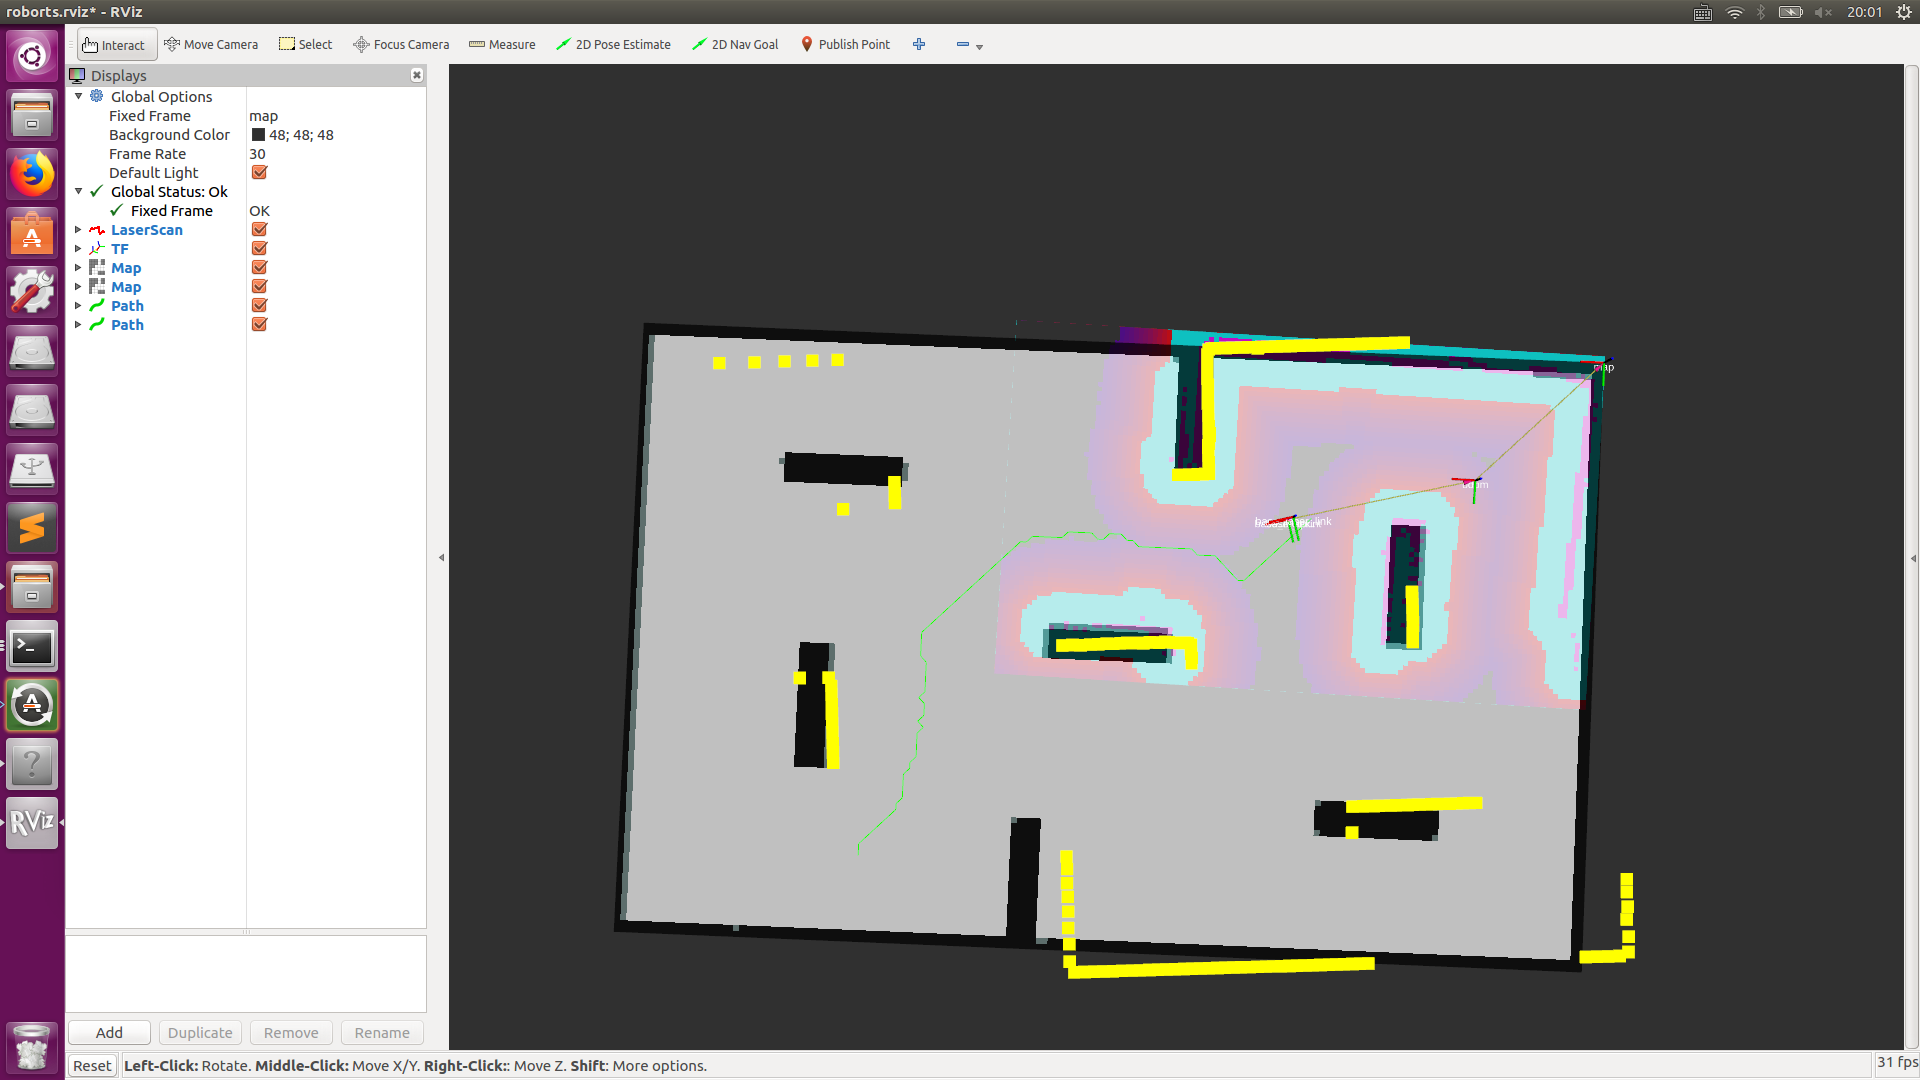
\includegraphics[width=0.80\textwidth]{figures/rviz.jpg}
  \caption{RVIZ界面}\label{rviz}
\end{figure}

\begin{figure}[ht]
  \centering
  % Requires \usepackage{graphicx}
  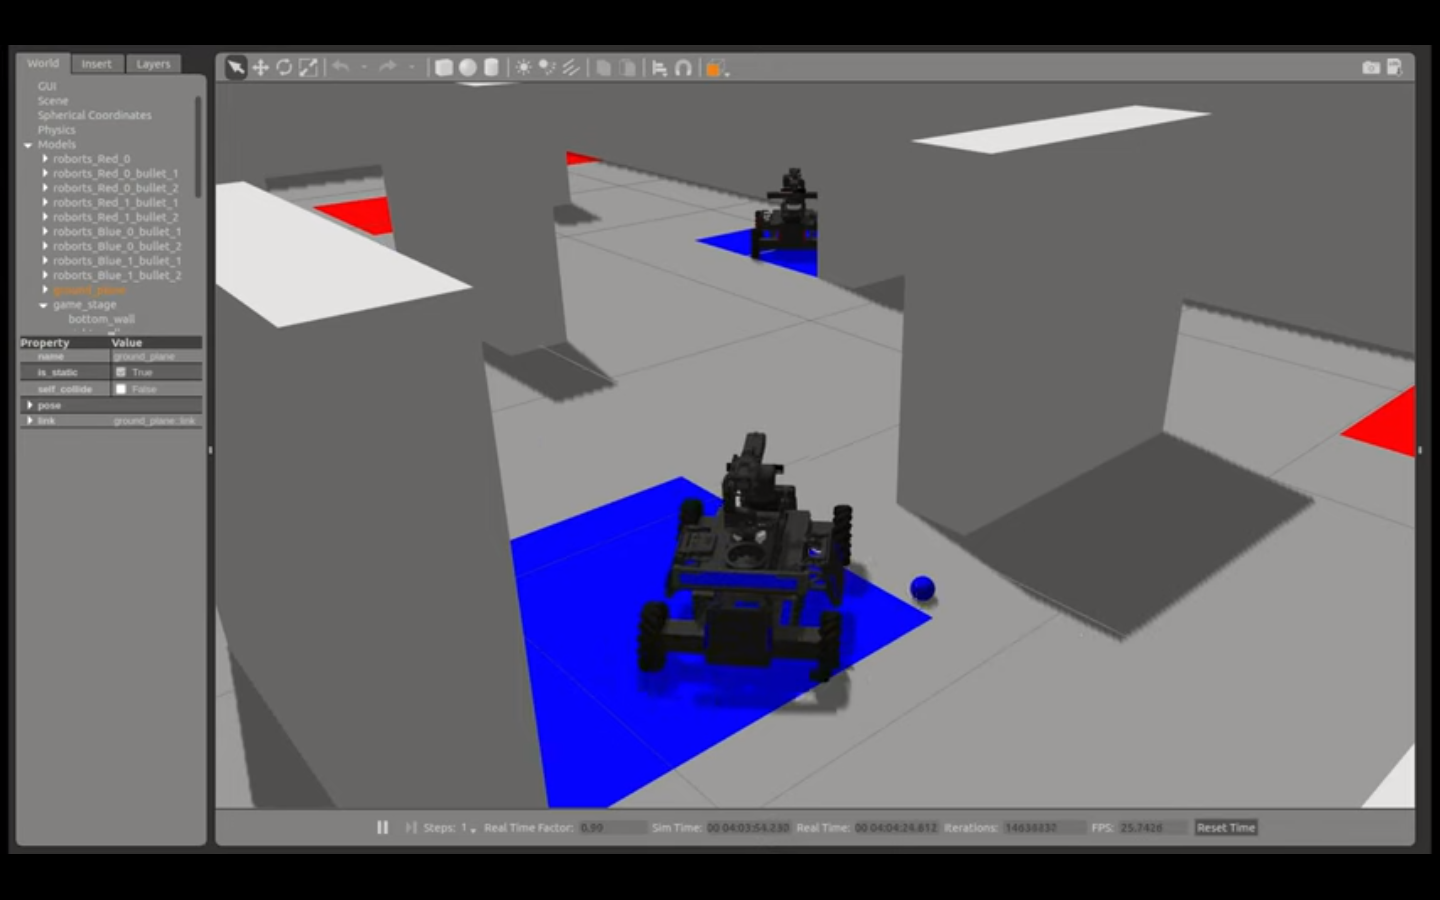
\includegraphics[width=0.80\textwidth]{figures/gazebo.png}
  \caption{Gazebo物理仿真}\label{gazebo}
\end{figure}

\section{真实环境}
我们在真实环境中使用的轮式机器人如图\ref{realrobot}所示。在真实环境中的深度强化学习训练具有比在虚拟环境下训练更具挑战性的问题:
\begin{enumerate}
  \item 必须选择适当的策略或者值函数表示,以便实现对物理硬件实用的训练时间。
  \item 必须提供实例演示来初始化策略并减轻训练期间的安全问题。
  \item 必须考虑到轮式机器人在真实世界的感知、通信和控制时延。
\end{enumerate}

针对安全问题,我们在进行真实环境下的实验时,进行一下设置以保证训练过程安全有效:
\begin{enumerate}
  \item 训练时,靶车即敌方机器人由人类操作员操作,以保证轮式机器人与场地人员安全。进行测试时,靶车由如图\ref{state}所示的确定性有限状态机控制作为实验基线。
  \item 训练时,轮式机器人在硬件上设置安全阈值和异常中断阈值,如表\ref{safty}。核查控制代码,使其控制论机器人的过程中,各安全项目的理论值在安全阈值以内。创建一个ROS结点,轮询安全项目数值,如果有超过异常中断阈值,则记录异常数值并终止轮式机器人运动。
  \item 训练时,使用远程桌面VNC控制轮式机器人。除操作员以外,无关人员禁止进入训练场地。
\end{enumerate}

针对时延问题,我们使用多智能体异步训练方法以求轮式机器人智能体能够克服物理时延带来的问题。

\begin{figure}[ht]
  \centering
  % Requires \usepackage{graphicx}
  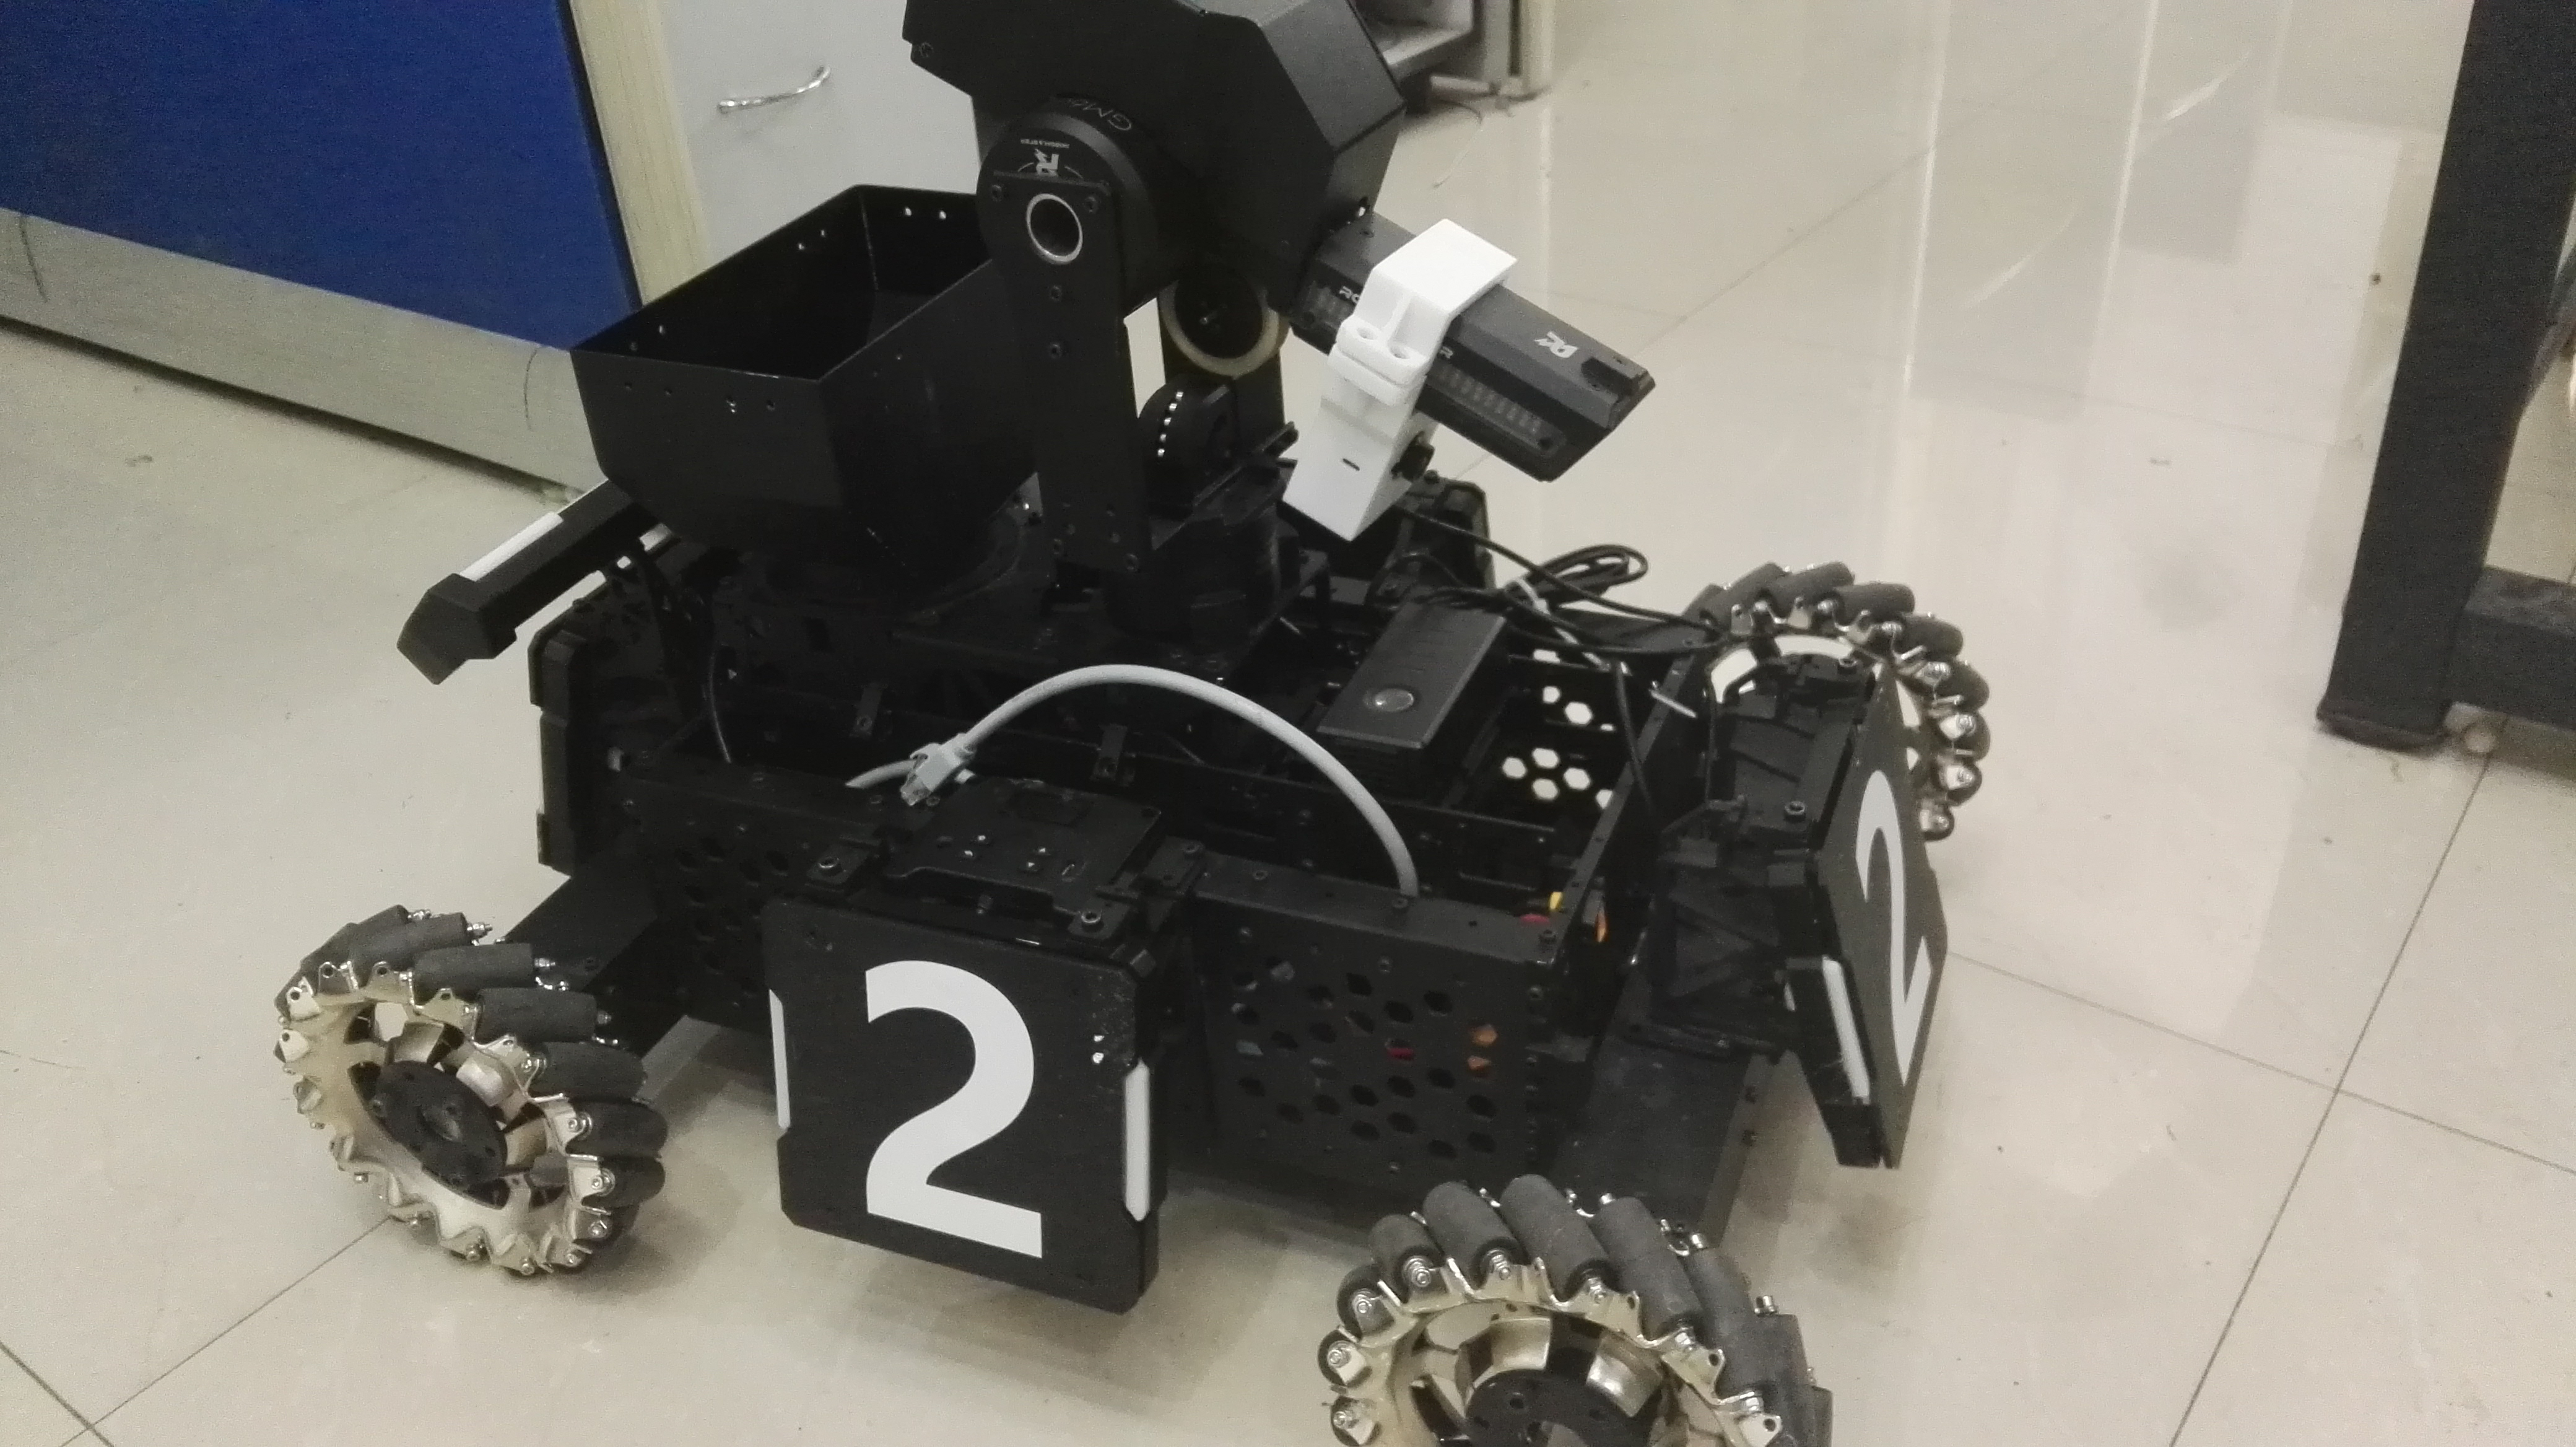
\includegraphics[width=0.80\textwidth]{figures/robot.jpg}
  \caption{轮式机器人实物}\label{realrobot}
\end{figure}

\section{奖励函数定义}
通过使用OpenAI gym标准的接口,实现ROS各个功能模组与决策系统的交互。通过串口向上位机发送轮式机器人的基本信息,轮式机器人智能体能够获得如比赛时间$t$、血量$h$、功率、里程计、速度、发射机构状态和遭受伤害的方向$d$等状态信息。通过传感器、定位算法(AMCL),轮式机器人智能体能够感知到自身位置与底盘偏航角$\left( x, y, \varphi \right)$。 通过目标识别算法(SSD-mobilenet),轮式机器人可以感知到敌人的位置$\left( x_e, y_e\right)$。

轮式机器人智能体所做出的动作包含下一步的目标位置与底盘偏航角$\left( x', y', \varphi' \right)$,或者相应的速度$\left( v_x, v_y, \omega \right)$,或加速度$\left( a_x, a_y, b \right)$,和发射机构云台的开火角度$\left( \theta, \psi \right)$。即云台俯仰角pitch、云台偏航角yaw。

考虑到与现有通信协议与控制算法整合,云台发射机构交由自动打击系统单独控制,打击策略为发现目标即开火,同时矫正云台姿态,智能体负责底盘运动的决策。最终定义状态$s$和动作$a$:
\begin{equation}
s = \left( x, y, \varphi, x_e, y_e, h, t, d \right),
\end{equation}
\begin{equation}
a = \left( x', y', \varphi' \right).
\end{equation}

奖励函数为:
\begin{equation}\label{reward}
r =
\begin{cases}
-1,  & \text{每受到一点伤害} \\
1, & \text{敌方轮式机器人出现在视野内} \\
10, & \text{获得增益buff}.
\end{cases}
\end{equation}

\section{代码设计}
\begin{figure}[ht]
  \centering
  % Requires \usepackage{graphicx}
  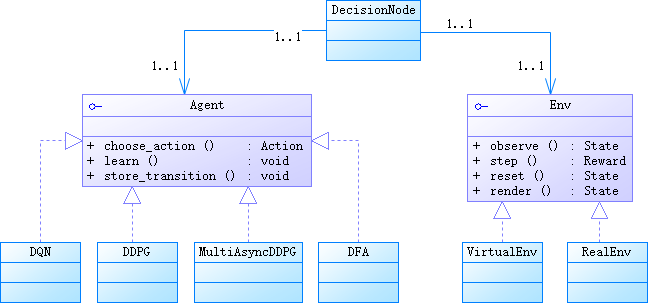
\includegraphics[width=\textwidth]{figures/classchart.png}
  \caption{轮式机器人决策系统类图}\label{classchart}
\end{figure}

\begin{figure}[ht]
  \centering
  % Requires \usepackage{graphicx}
  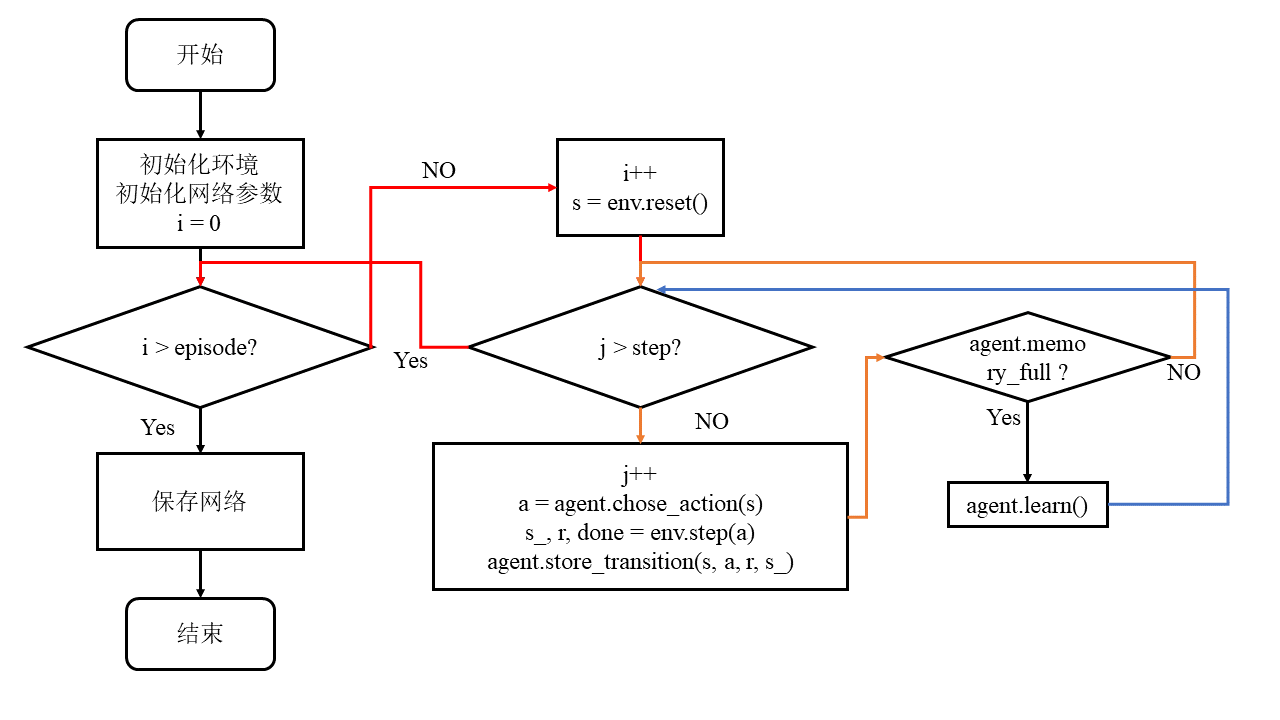
\includegraphics[width=\textwidth]{figures/flowchart.png}
  \caption{训练过程流程图}\label{flowchart}
\end{figure}

智能体类agent与环境类env结构与接口,如图\ref{classchart}所示。我们按照OpenAI gym接口规范标准,将智能体和与智能体直接交互的环境封装为接口。

环境类env隐藏了与轮式机器人感知、控制和通信等细节,从而使智能体类agent只需要关心与环境类env的交互,即接收一个状态$s$,做出相应的动作决策$a$。同时,智能体类agent隐藏了自主决策算法的训练和执行细节,环境类只需要关心执行智能体类输出的动作决策$a$。这样的结构允许我们在仿真环境到真实环境下的平滑过渡,同时也支持不同网络结构的深度强化学习算法的切换,甚至是使用非强化学习算法,如确定性有限状态机或遗传算法等启发式搜索算法。

针对深度强化学习,对于每一个情节(episode),我们设置最大步长数。训练时,轮式机器人智能体达到步长后即终止本次情节,重置环境,进入下一个情节的训练。训练过程如图\ref{flowchart}所示。

\subsection{Deep Q-learning}
使用Tensorflow构建DQN网络,网络结构如图\ref{dqnnet}所示。其中当前网络和目标网络均为三层全连接层神经网络,每层的神经元数分别为64,128,256,隐藏层的激活函数为Relu,输出层的激活函数为Tanh。
\begin{figure}[b]
  \centering
  % Requires \usepackage{graphicx}
  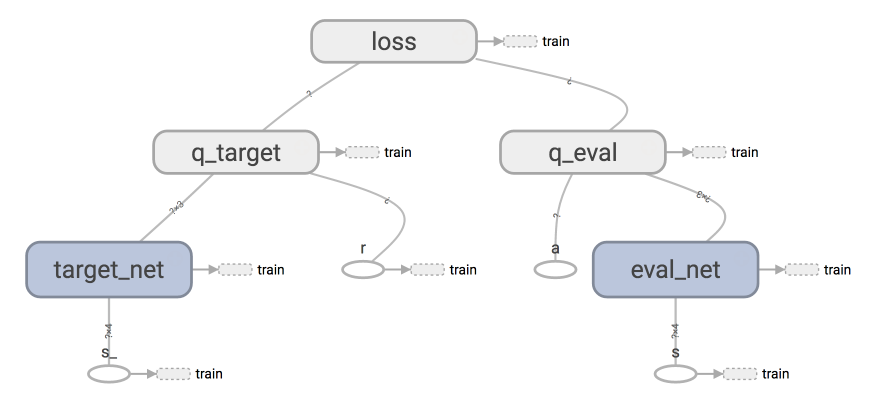
\includegraphics[width=0.80\textwidth]{figures/dqnnet.png}
  \caption{DQN网络结构图}\label{dqnnet}
\end{figure}

\subsection{Deep Deterministic Policy Gradient}
使用Tensorflow构建DDPG网络,网络结构如图\ref{ddpgnet}所示。其中当前网络和目标网络同构。网络中演员为三层全连接层神经网络,每层的神经元数分别为64,128,256,隐藏层的激活函数为Relu,输出层的激活函数为Tanh;评论家网络为三层全连接神经网络,每层的神经元数分别为64,128,1,输出标量评价值,即Q值的估计。
\begin{figure}[ht]
  \centering
  % Requires \usepackage{graphicx}
  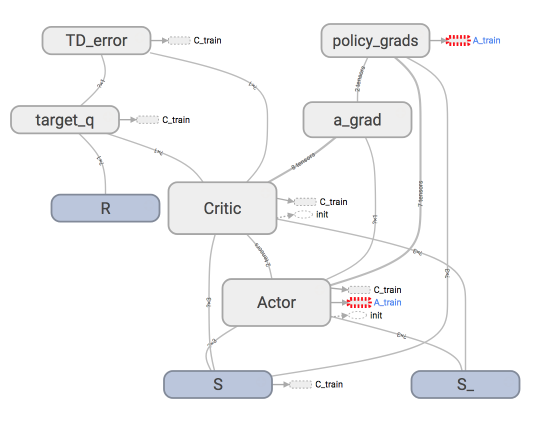
\includegraphics[width=0.80\textwidth]{figures/ddpgnet.png}
  \caption{DDPG网络结构图}\label{ddpgnet}
\end{figure}

\subsection{多智能体异步DDPG}
使用Tensorflow构建多智能体异步DDPG,其网络结构图与DDPG保持一致。在Gazebo仿真环境中,一次使用四台轮式机器人智能体进行对抗训练,如图\ref{multia}所示。
\begin{figure}[ht]
\centering
\subfigure{
\begin{minipage}[t]{0.40\linewidth}
\centering
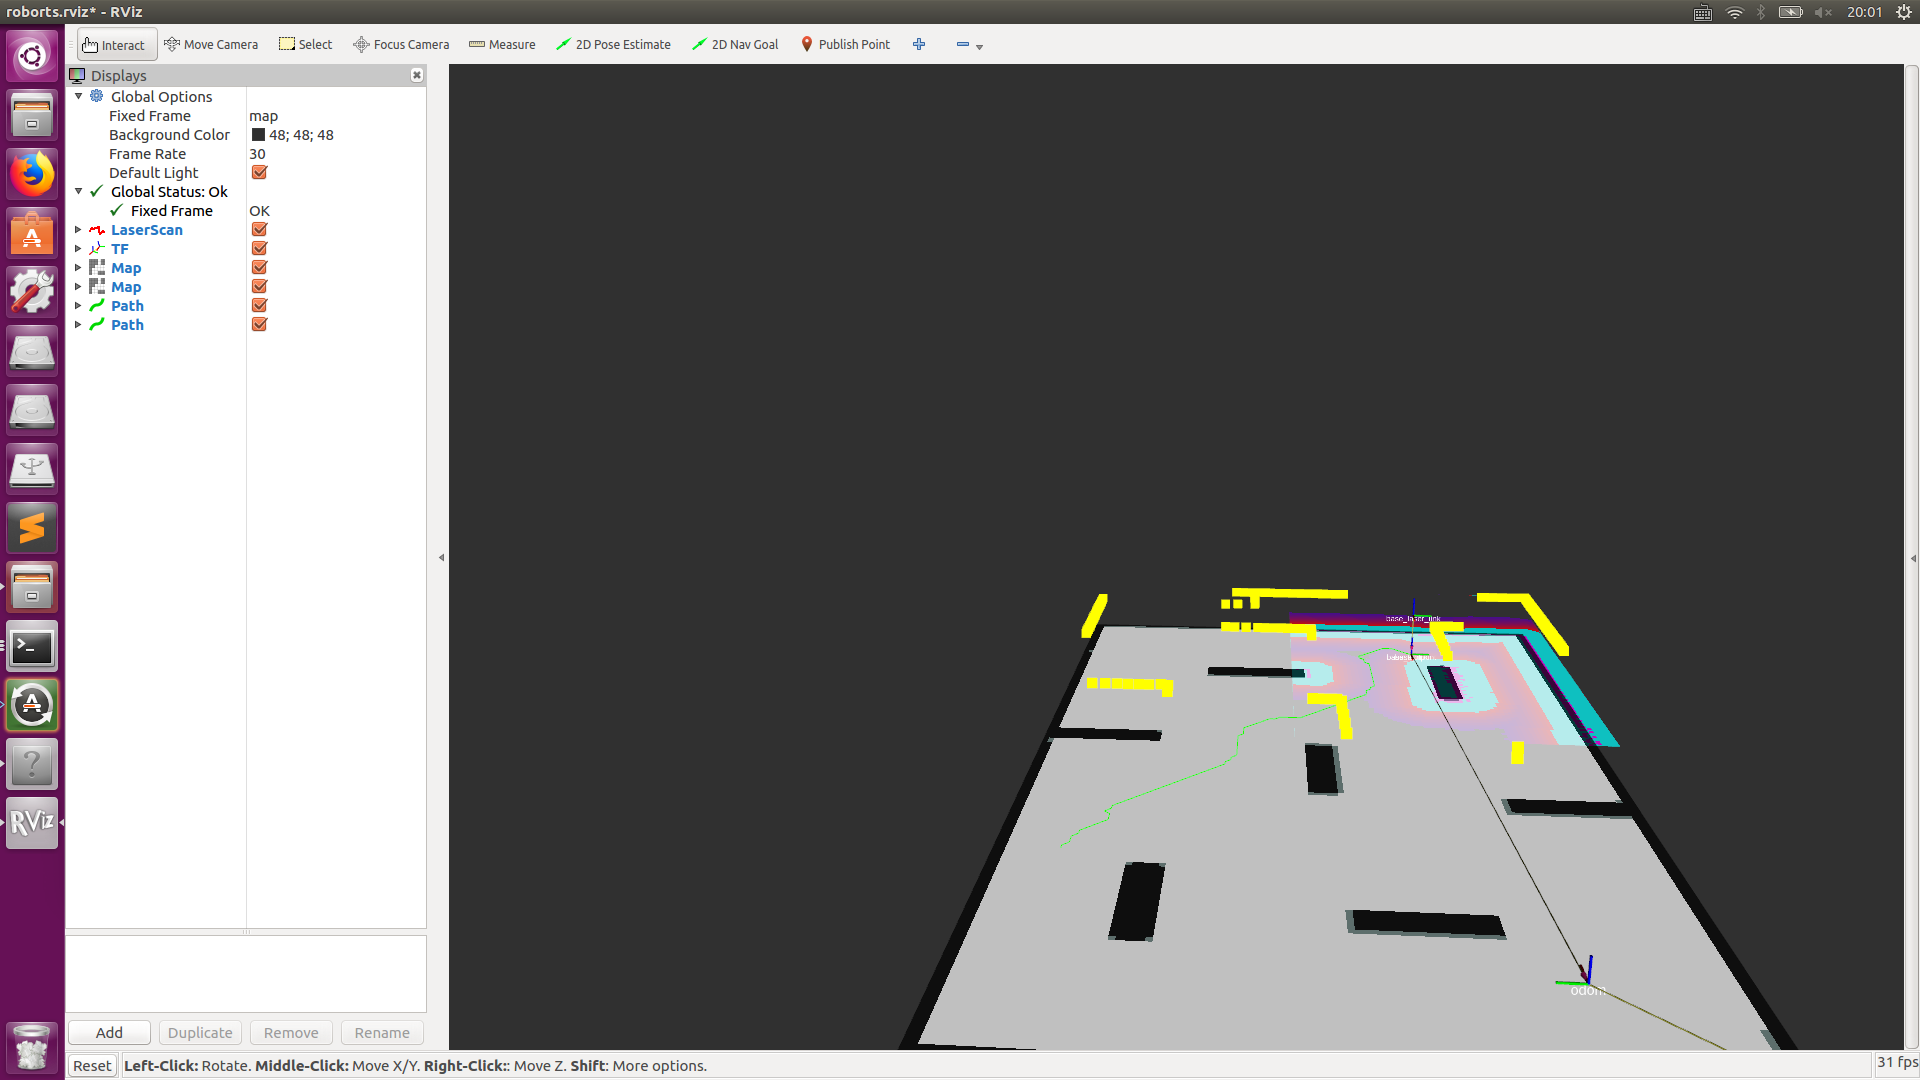
\includegraphics[width=2in]{rviz1.jpg}
\end{minipage}
}
\subfigure{
\begin{minipage}[t]{0.40\linewidth}
\centering
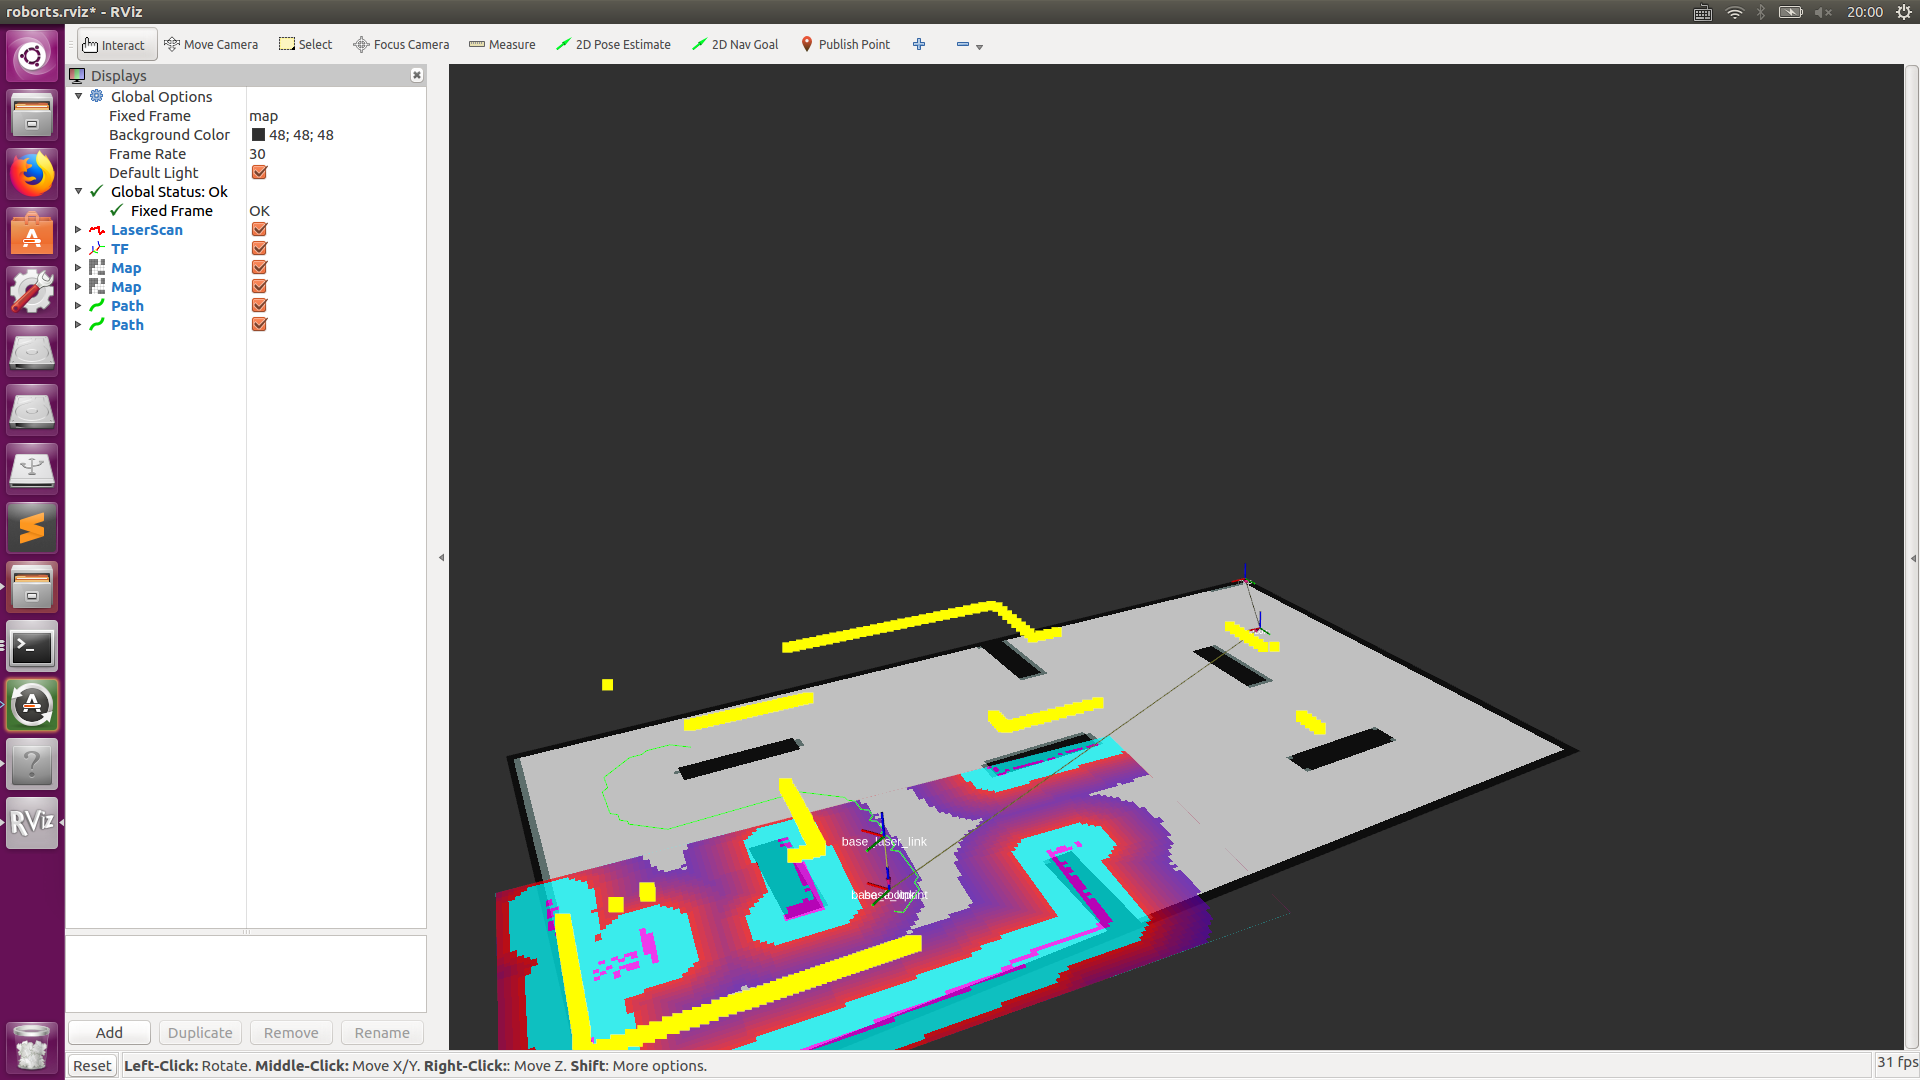
\includegraphics[width=2in]{rviz2.jpg}
\end{minipage}
}
\subfigure{
\begin{minipage}[t]{0.40\linewidth}
\centering
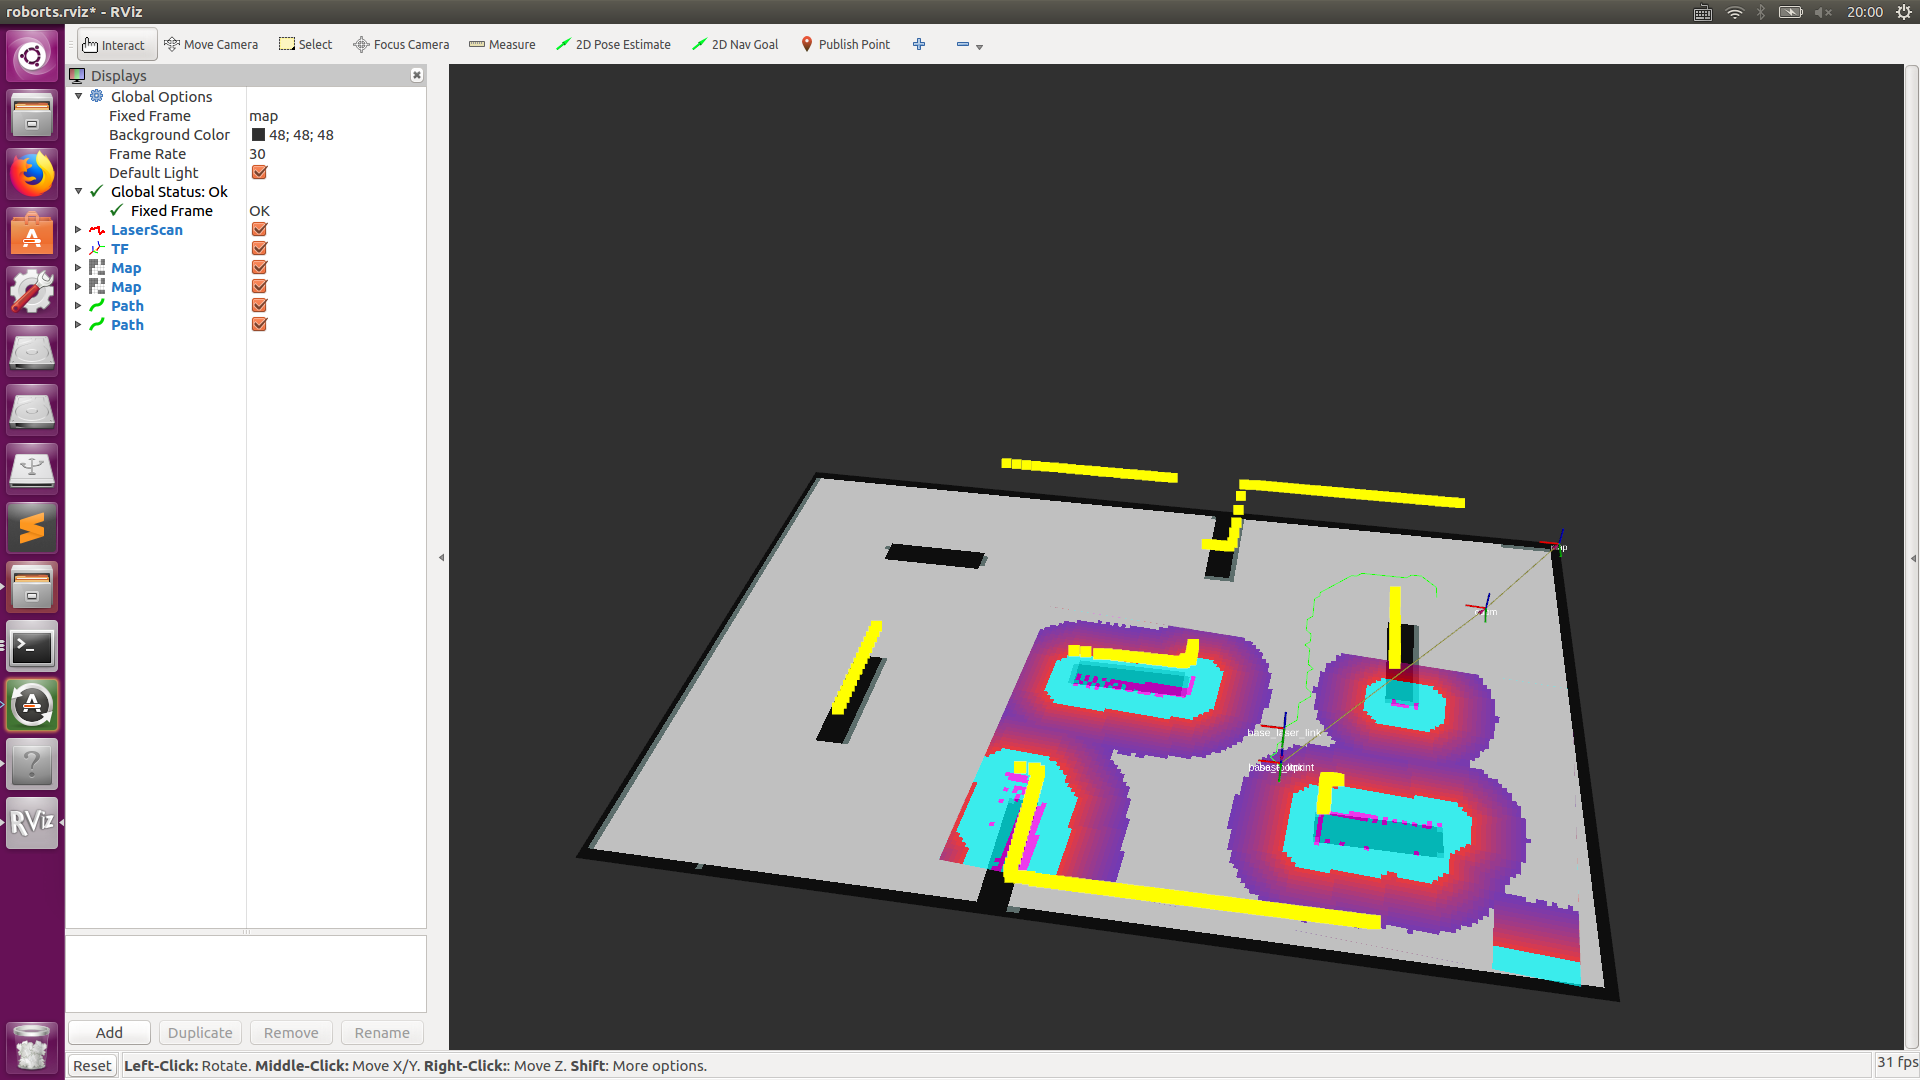
\includegraphics[width=2in]{rviz3.jpg}
\end{minipage}
}
\subfigure{
\begin{minipage}[t]{0.40\linewidth}
\centering
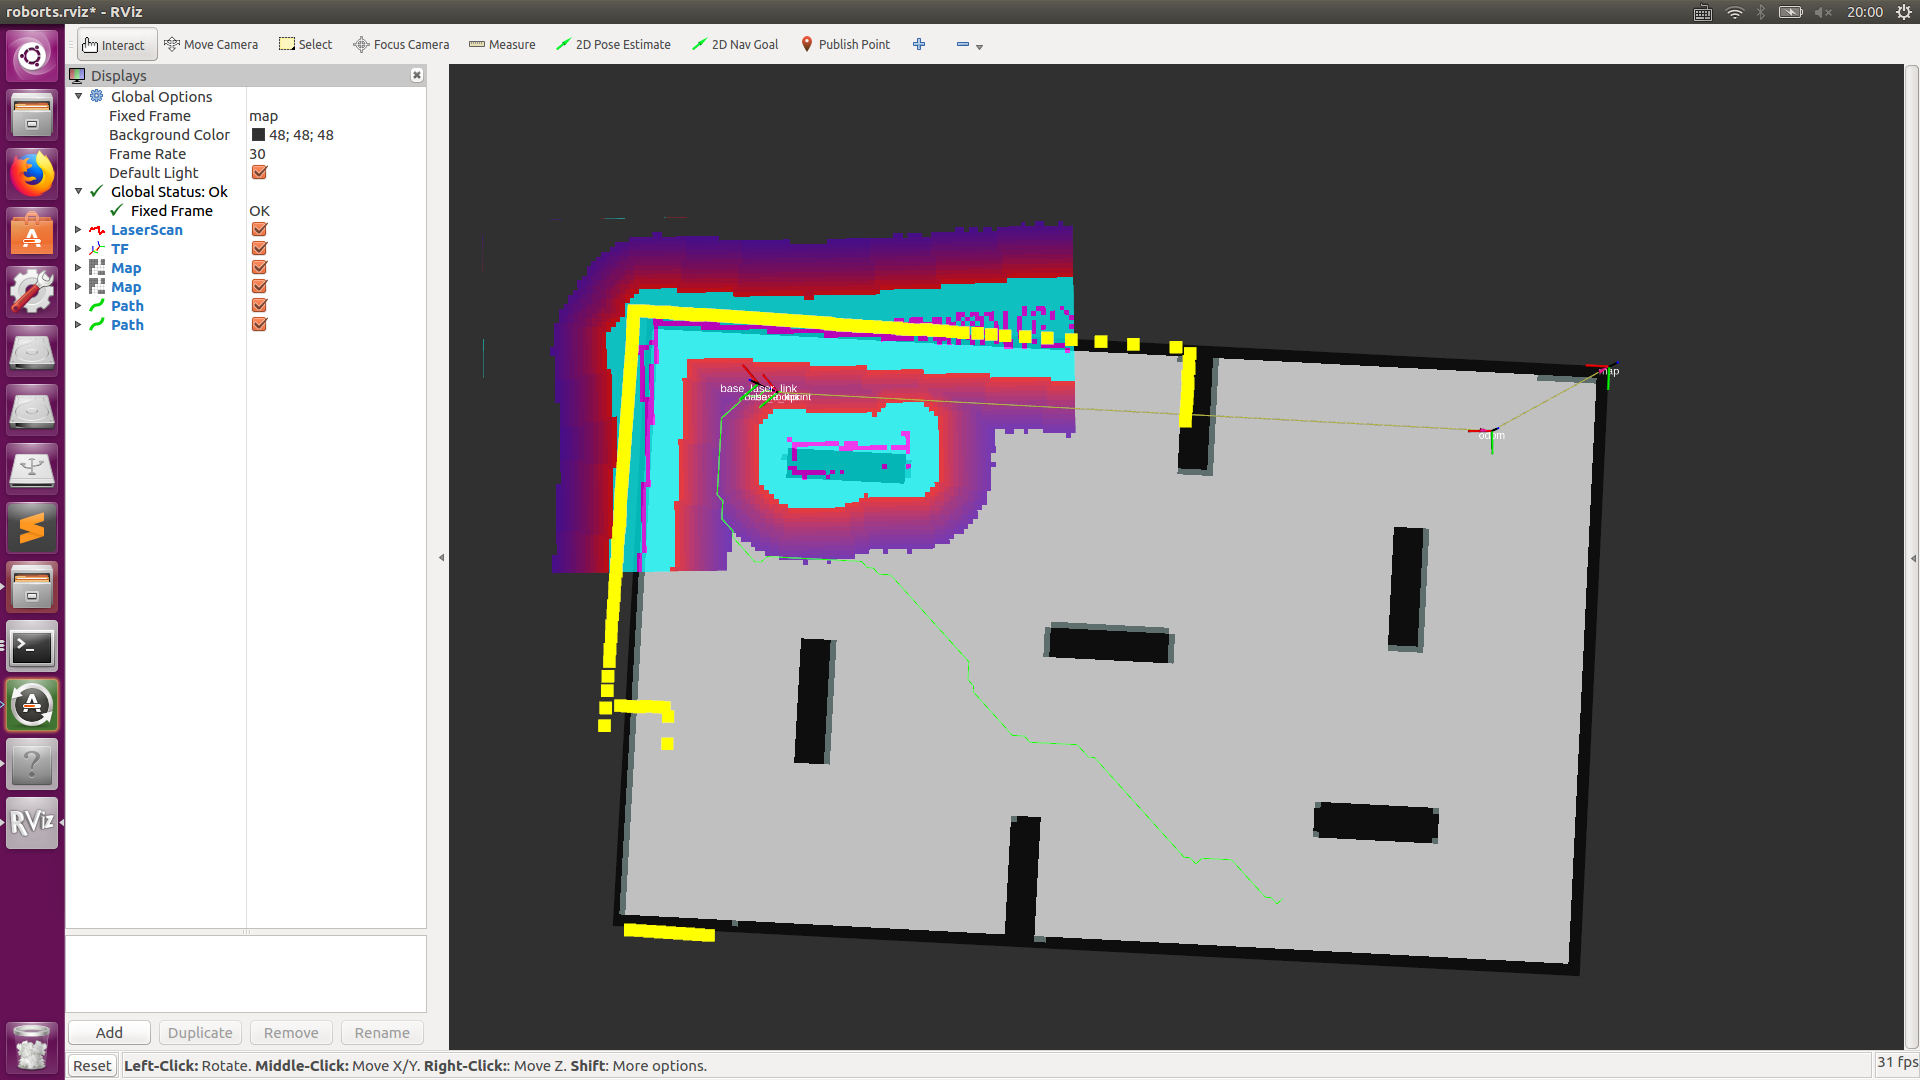
\includegraphics[width=2in]{rviz4.jpg}
\end{minipage}
}
\caption{多智能体异步DDPG训练}\label{multia}
\end{figure}

\section{实验结果}
\subsection{仿真实验结果}
在仿真环境下,我们使用上述定义的参数,应用DQN,DDPG,多智能体异步DDPG,在Gazebo仿真平台上训练全自主轮式机器人。使用的超参数有:
\begin{itemize}
  \item 情节数,episode:500。
  \item 最长步数,step:300。
  \item 折扣参数,$\gamma$:0.90。
  \item 学习率,learning rate:1e-3。
  \item 回放记忆长度,reply memory:30000。
  \item 批处理长度,batch size:50。
\end{itemize}

应用三种不同算法在仿真环境下的表现如图\ref{performance}所示。其中图\ref{accumulatedreward}表示仿真环境下轮式机器人在训练中共获得的奖励累加值,图\ref{averagereward}表示仿真环境下轮式机器人的步长平均奖励,即奖励累加值除以当前进行过的步长,可以是作为奖励期望的估计。由奖励设置式\ref{reward} 可推知,步长平均奖励近似于敌方出现在轮式机器人视野的概率,我们可将之称为锁定率。在图中我们可以看出,在DQN、DDPG 以及多智能体异步DDPG三种深度强化学习算法中,多智能体异步DDPG算法收敛速度较快,其模型锁定率能够达到18\%以上,而DDPG和DQN分别收敛在9\%和4\%左右。

\begin{figure}[hb]
  \centering
  % Requires \usepackage{graphicx}
  \subfigure[仿真环境下轮式机器人的累积奖励]{
  \label{accumulatedreward}
  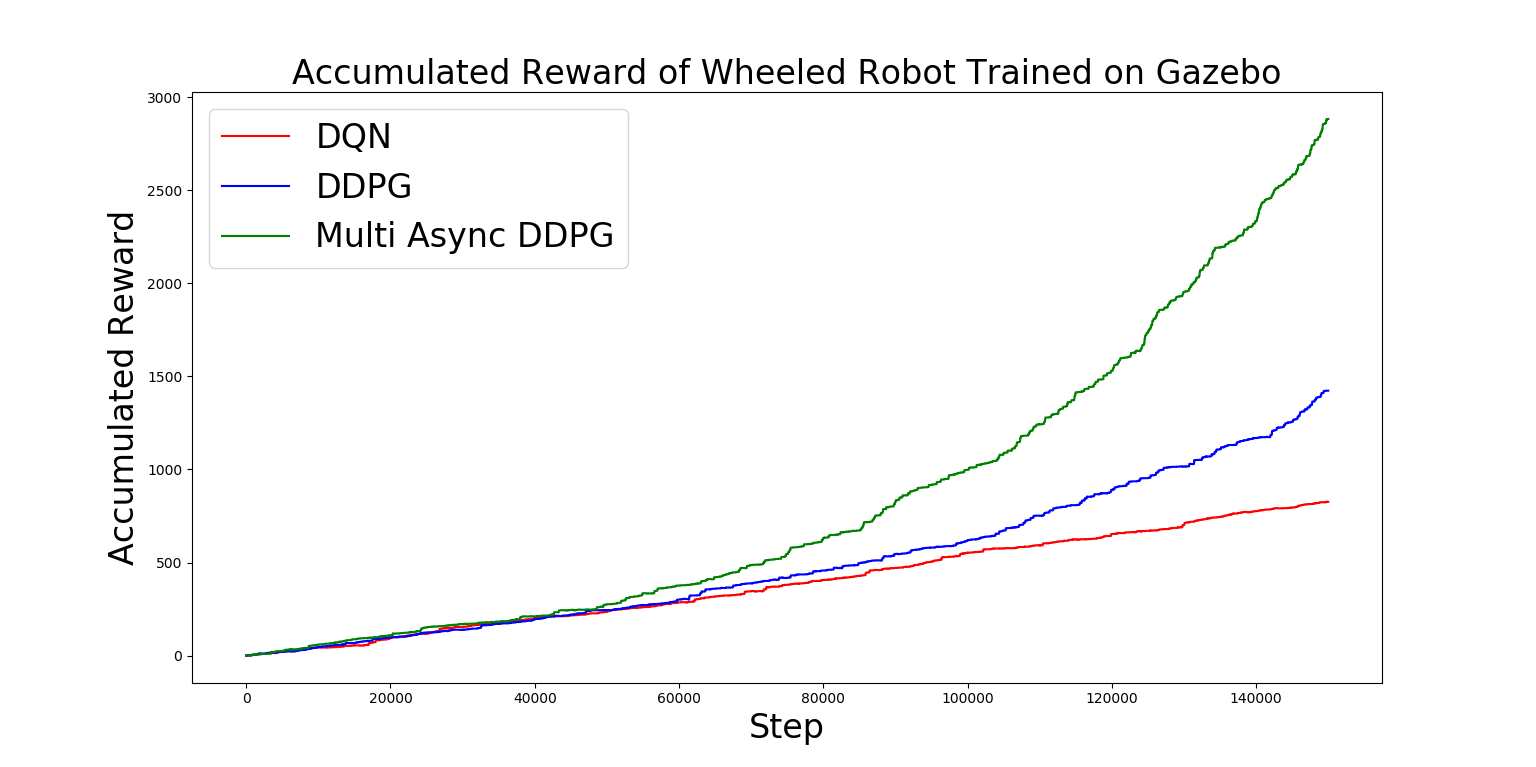
\includegraphics[width=0.80\textwidth]{figures/accumulatedreward.png}
  }
  \subfigure[仿真环境下轮式机器人的步长平均奖励]{
  \label{averagereward}
  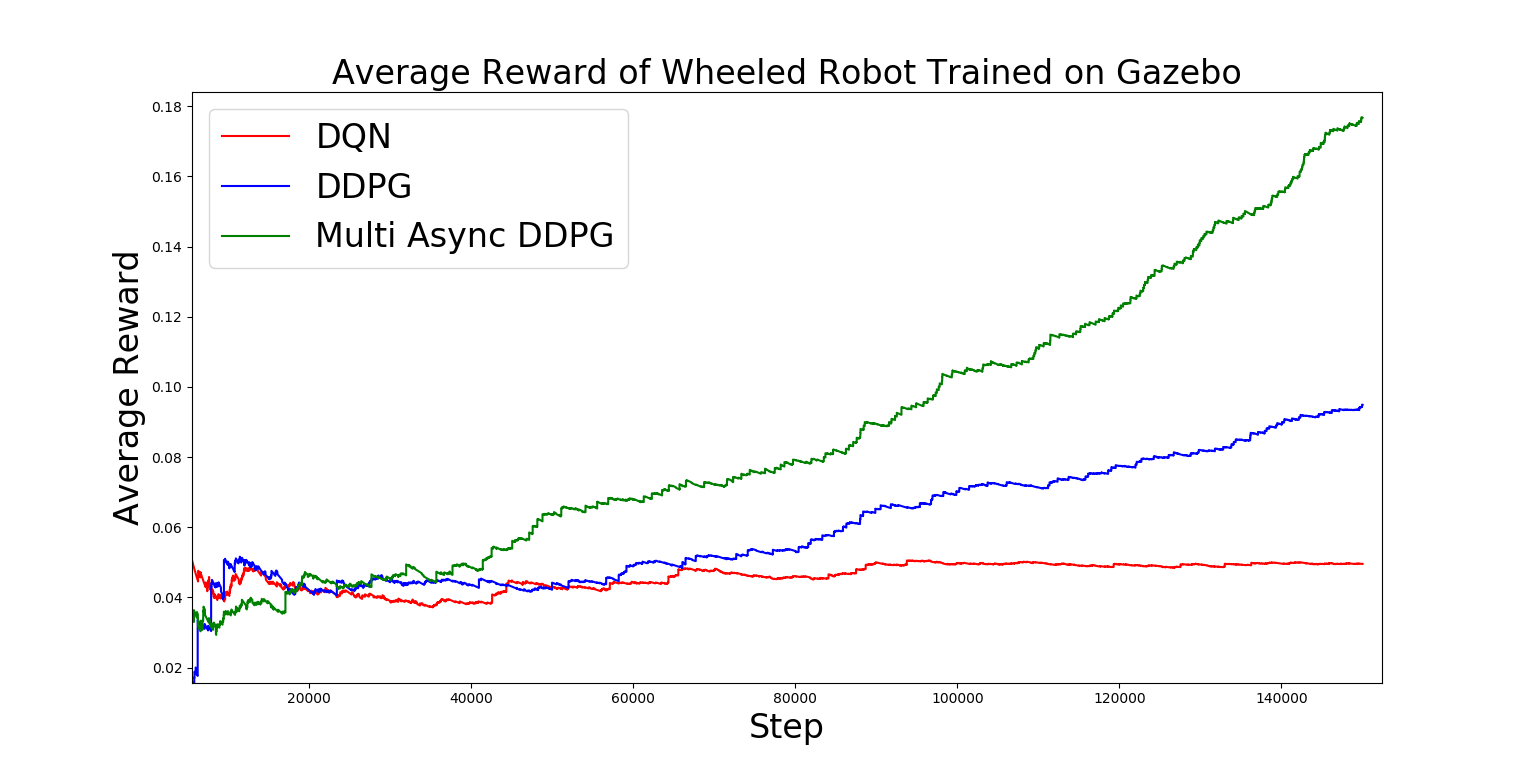
\includegraphics[width=0.80\textwidth]{figures/averagereward.png}
  }
  \caption{仿真环境下轮式机器人的训练表现}\label{performance}
\end{figure}

\subsection{真实环境下对抗结果}
在真实环境下,我们使用确定性有限状态机作为基线与三种不同算法训练的轮式机器人智能体各进行8次实际对战,在120s的比赛时间内的比赛结果如图\ref{result}所示。图中黑色直线为失败线,分布在黑色直线上的点即为血量被敌方轮式机器人伤害殆尽而结束比赛;棕色线为胜利线,分布在棕色线上的点即为在保佑一定血量的情况下使敌方轮式机器人血量消耗殆尽;橙色线为优势线,即在比赛时间结束时,敌我双方都没有击败对方,此时处于优势线右侧的点表示在比赛结束时,我方轮式机器人智能体保有血量高于敌方。
由图中结果可以发现多智能体异步DDPG算法和DDPG算法在真实环境下与敌方对抗时各有三次取得优势,实际上的表现相近,而DQN则很难取得优势。这说明了多智能体异步DDPG算法实际上是DDPG算法的快速收敛版。通过多智能体异步的方法部分克服了时延问题和采样速度较慢的问题。
\begin{figure}[ht]
  \centering
  % Requires \usepackage{graphicx}
  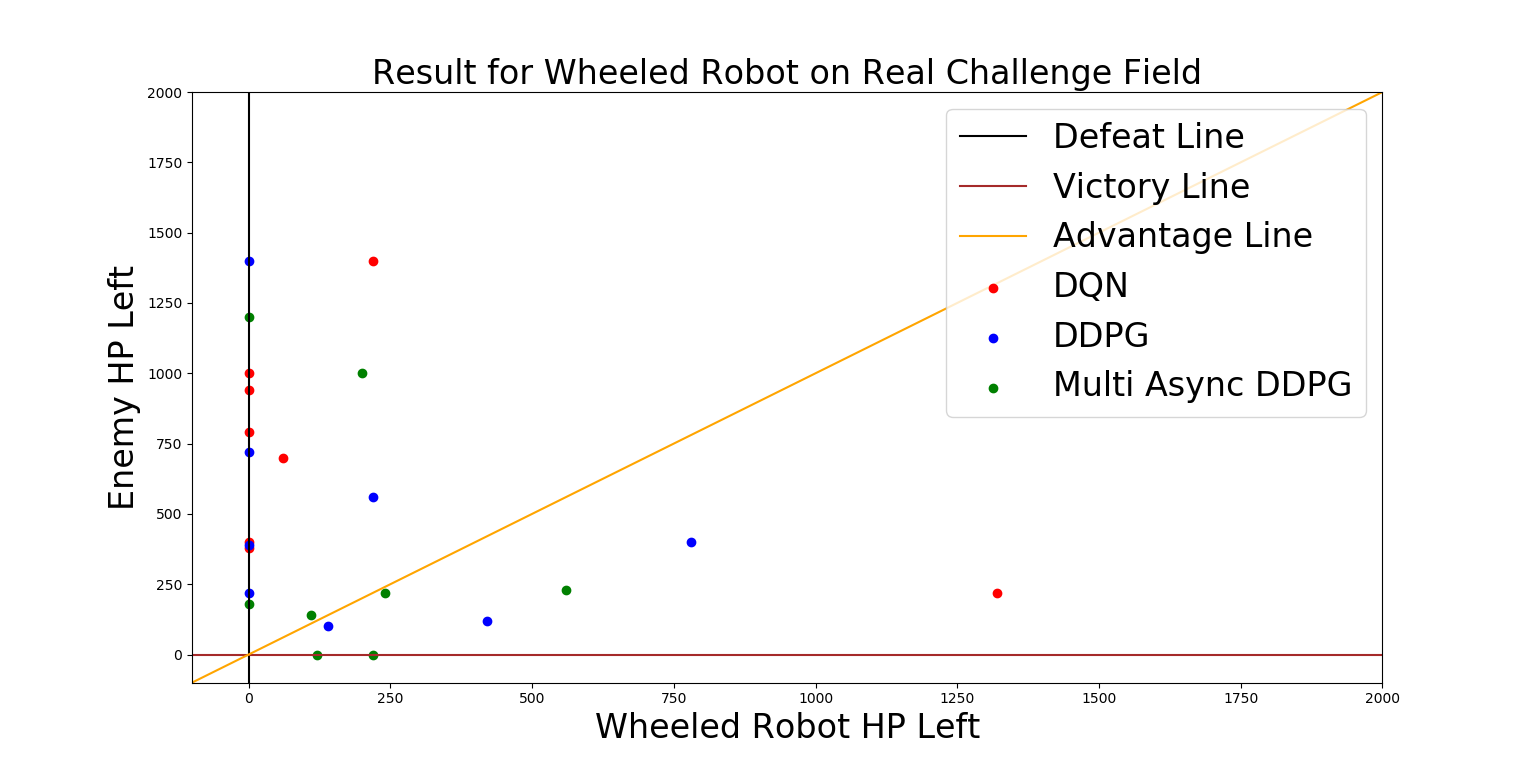
\includegraphics[width=0.80\textwidth]{figures/result.png}
  \caption{真实环境下轮式机器人对抗结果}\label{result}
\end{figure}
